\section{Schwierigkeiten von Vektoruhren}
\subsection{Effizienten Speicherung von Vektoruhren}
% Paper: Concerning the size of clocks 
%        Plausible Clocks Constant Size Logical Clocks for Distributed Systems
Vektor Uhren sind eine relativ einfache und effektive Lösung kausale Ordnung in einem verteilten System herzustellen.
Ihre Definition beherbergt jedoch ihren größten Nachteil.
Die Größe einer Uhr ist nicht konstant.
Für ein verteiltes System mit $n$ Prozessen benötigt eine Vektor Uhr $n$ Komponenten i.d.R. Integer-Zahlen.
Die Folge ist, dass für ein großes verteiltes System alle Vektor Uhren einen entsprechend hohen Speicherbedarf haben.
Dies wirkt sich zum einen negativ auf den Speicherverbrauch der einzelnen Prozesse aus, da je nach Implementierung mehrere Uhren gespeichert werden müssen.
Außerdem fügen die großen Vektor Uhren einen Overhead zu den Nachrichten hinzu und belasten somit den Übertragungsweg.
Offensichtlich ist die Länge der Vektor Uhr direkt proportional zur Anzahl der Prozesse.
Somit skalieren Vektor Uhren schlecht \cite{torres1999plausible}.

Charron-Bost \cite{charron1990concerning} hat bewiesen, dass es innerhalb eines Systems bestehend aus $n$ Nodes immer eine mögliche Kombination an Ereignissen geben kann, bei der die Kausalität ausschließlich mit Vektor Uhren der Länge $n$ erfasst werden kann.
Von daher müssen für alle theoretisch vorkommenden Prozesse innerhalb des Systems eine Komponente in der Uhr reserviert werden.
Dies beinhaltet alle aktuellen Prozesse und auch zukünftige Prozesse die möglicherweise ausgeführt werden könnten.
Es ist natürlich schwer im voraus zu entscheiden wie viele Prozesse potentiell ausgeführt werden und ist daher im Allgemeinen nur bei statischen Systemen gegeben, bei denen also  bei denen also die Anzahl der Prozesse konstant ist.
Daher muss theoretisch eine Vektor Uhr mit einer statischen Länge von $n$ verwendet werden.
Im Folgenden werden verschiedene Verfahren vorgestellt um die Länge von Vektor Uhren zu reduzieren.

Ein pragmatisches Vorgehen um die Länge einer Vektor Uhr in einer annehmbarer Größe zu halten wurde von Amazon in ihrer Dynamo Datenbank \cite{decandia2007dynamo} verfolgt.
Hierbei wird die Länge durch folgendes Kürzungsschema reduziert:
Zu jeder Komponente in der Vektor Uhr wird neben dem Zähler noch die Prozess ID und ein Zeitstempel gehalten.
Der Zeitstempel gibt den Zeitpunkt an, zudem der entsprechende Prozess zuletzt den Datensatz aktualisierte.
Erreicht die Länge der Vektor Uhr einen bestimmten Schwellwert, werden die Komponenten mit den ältesten Zeitstempel aus der Uhr entfernt.
Dieses Verwerfen von Daten kann dazu führen, dass in gewissen Situationen die Kausalität nicht mehr komplett hergestellt werden kann.
Nach eigenen Angaben von \etal{DeCandia} \cite{decandia2007dynamo} trat dieses Problem im Produktiveinsatz jedoch nicht auf und wurde daher nicht weiter analysiert.

\etal{Singhal} \cite{singhal1992efficient} stellten ein einfaches Verfahren vor um den Overhead bei der Nachrichtenübertragung im Durchschnitt zu verringern.
Ihre Technik basiert auf der empirischen Beobachtung, dass nur wenige Prozesse häufig miteinander kommunizieren.
Außerdem ist es wahrscheinlich, dass zwischen zwei aufeinanderfolgend Sende-Ereignisse von Prozess $P_i$ zu $P_j$ nur wenige Komponenten der Vektor Uhr sich ändern.
In diesem Fall ist es unnötig die komplette Uhr mit jeder ausgehenden Nachricht von $P_i$ zu $P_j$ zu übertragen.
Es ist ausreichend nur die Komponenten zu übertragen die sich geändert haben.
Konkret kann bei einer gegeben Uhr $VC$ für jede geänderte Komponenten ein Tupel aus $(a, VC[a])$ übertragen werden, wobei $a$ dem Index des Prozess innerhalb der Uhr entspricht.
Werden Vektor Uhren nach dieser Technik übertragen kann die zu übertragene Datenmenge reduziert werden.
Dabei wird jedoch der lokale Speicherbedarf eines Prozesses erhöht, da dieser zusätzlich speichern muss welche Werte zuletzt zu welchen Prozess geschickt wurden.
Anhand den gespeicherten Vektoren kann er die entsprechenden Tupel auswählen, die an eine Nachricht mit angehängt werden müssen.

\begin{figure}[ht]
    \centering
    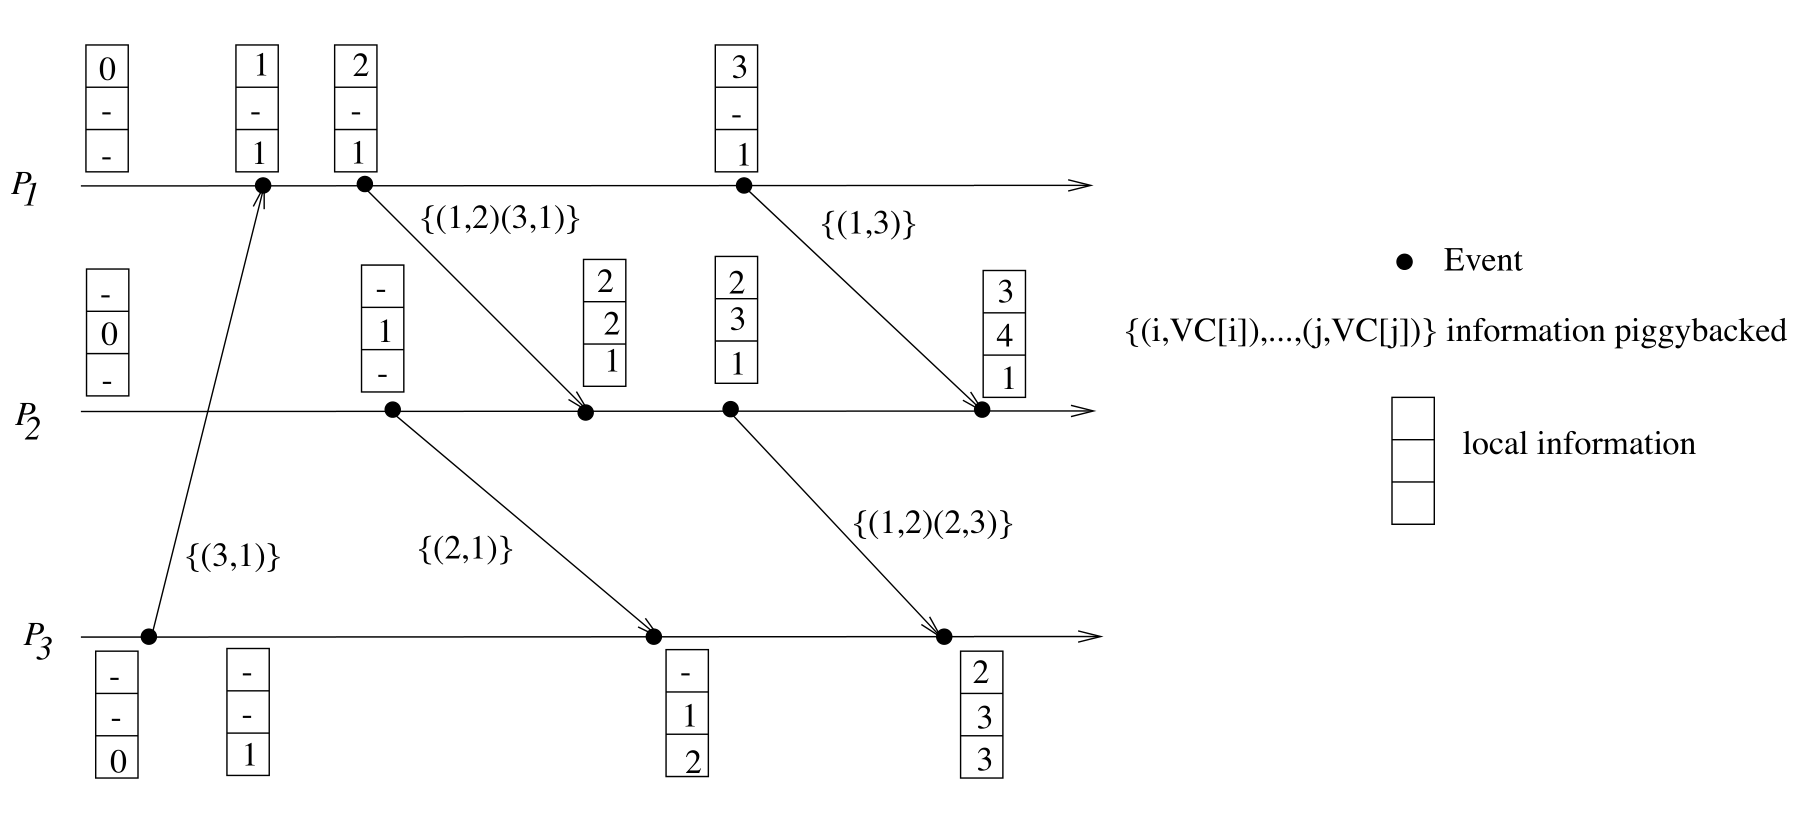
\includegraphics[width=1\textwidth]{Singhal.png}
    \caption[Kommunikaiton nach Singhal]{Ablauf der Kommunikation dreier Prozesse nach dem Verfahren von \etal{Singhal}.}
    Quelle: Nachgezeichnet aus \cite{Baldoni:2002:FDC:1435723.1437765}
    \label{fig:singhal}
\end{figure}

Bisher wurde immer angenommen, dass die Anzahl der Prozesse innerhalb eines Systems konstant ist.
Dies ist jedoch selten der Fall, in der Regel werden Prozesse häufig gestartet und beendet.
Die Folge ist, dass bei einer naiven Implementierung der Vektor Uhr für jeden jemals ausgeführten Prozess eine Komponente in der Uhr reserviert werden muss.
In dynamischen Systemen kann dies dazu führen, dass die Uhren schnell eine tragbare Größe überschreiten.
Es ist daher wünschenswert Vektor Uhren für solche dynamische Systeme zu optimieren.

Fridge \cite{fidge1991logical} stellte ein Modell vor bei dem eine variable Anzahl an Prozess-IDs verwendet wird.
Hierbei müssen die Prozess-IDs innerhalb des Systems eindeutig sein.
Beim Start eines Prozesses wird ihm eine ID zugewiesen.
Die ID eines terminierten Prozesses wird jedoch nicht freigegeben.
Damit die IDs solcher Prozesse freigegeben werden können, müssen allen anderen Prozesse die Terminierung bekannt sein.
Ist dies nicht gegeben, darf die ID nicht aus der Vektor Uhr entfernt werden.
Diese Art von Garbage Collection wird in \cite{richard1998efficient} verwendet.
Alle Verfahren dieser Art haben jedoch das Problem, dass IDs von terminierten Prozessen nicht wiederverwendet werden können und die Bereinigung der Uhr von terminierten Prozessen durch einen einzigen unerreichbaren Prozess bereits verhindert werden kann \cite{almeida2008treeclocks}.

% Hier würde Landes reinpassen

Wie gezeigt führt die Verwendung von globalen IDs zu neuen Problemen.
Es liegt somit nahe auf globale IDs gänzlich zu verzichten.
Aus dieser Überlegung heraus entwickelten \etal{Almeida} \cite{almeida2008treeclocks} eine Generalisierung von Vektor Uhren.
Die sogenannten \qq{Interval Tree Clocks} sind für dynamische Systeme ausgelegt und kommen dabei ohne globale IDs aus, indem jeder Prozess selbständig neue IDs erzeugen, löschen oder wiederverwenden kann, ohne das dabei auf eine globale Kommunikation zurückgegriffen werden muss.
Durch teilen und zusammenfassen von Prozess IDs wachsen und schrumpfen die Zeitstempel entsprechend zu der Dynamik des Systems.
Der Platzbedarf der Zeitstempel skaliert somit mit der Anzahl der Prozesse und wächst nur moderat an \cite{almeida2008treeclocks}.

% \cite{almeida2008treeclocks}
% landes dynamic clock

Ein in der Praxis relevantes Problem ist die Handhabung von Integer Überlaufen der Zählern innerhalb der Uhr.
In der Theorie werden die natürlichen Zahlen als Menge der möglichen Zählerwerte angenommen und haben somit keine Beschränkung.
Bei der Implementierung einer Vektor Uhr muss jedoch über die Darstellung der Vektorkomponenten entschieden werden.
In der Regel wird ein Integer Datentyp mit typischerweise 32 oder 64 Bit gewählt.
Dabei muss ein Kompromiss zwischen maximale Länge und Datenmenge die zu übertragen ist gefunden werden.
Wird das verteilte System lange genug ausgeführt oder treten hochfrequent Ereignisse auf, kann es durchaus passieren, dass die Bitgrenze des gewählten Datentyps erreicht ist und ein Overflow zur Folge ist.
Dabei springt der Zähler vom Maximalwert auf Null.
\etal{Yen} \cite{yen1997resetting} stellen hierzu ein Protokoll vor um die Uhren zurückzusetzen.
Wird dieses Schema implementiert kann bei manche Anwendungen darauf verzichtet werden die optimale Bitlänge der Vektorkomponenten zu bestimmen. Da lediglich ein geeigneter Auslöser für den Uhrenreset gefunden werden muss \cite{yen1997resetting}.
Ein allgemeingültiges Verfahren wurde von Baldoni \cite{baldoni1998positive} vorgestellt.

% cap:vectorclock
\subsection{Gleichzeitig abgesendete Nachrichten}
\label{lbl:consistency}
% Verteiltes System
% Replika
% Konsitenz 
consistency

% Strong
>
Causal
>
Eventual

Wie bereits in der Einführung erwähnt, existiert kein globaler Zustand in einem verteilten System.
Vielmehr wird die Vereinigung aller lokalen Zustände als globaler Zustand verstanden.
Voraussetzung hierzu ist, dass alle Prozesse zu einem gewissen Zeitpunkt den selben lokalen Zustand haben.

Konkret kann es sich bei einem globalen Zustand zum Beispiel um ein Datenfeld in einer verteilten Key-Value-Datenbank handeln.
Jedes Datenfeld kann durch einen eindeutigen Schlüssel aus der Datenbank ausgelesen werden.
Alle Prozesse halten eine Replikation dieser Schlüssel-Werte Paare.
Durch die Kopie hat sich die Identität der Entität nicht geändert, das heißt obwohl eine Kopie gemacht wurde, handelt es sich immer noch um das selbe Objekt.

Wird nun in einem Prozess dieses Datenfeld modifiziert, muss die Änderung allen anderen Prozessen bekannt gemacht werden, damit diese den neuen Wert annehmen können.
Solange die Prozesse nach einer Datenänderung unterschiedliche Werte haben, ist das System inkonsistent, da je nachdem an welchem Prozess die Entität abgefragt wird, ein abweichender Wert zurück gegeben werden kann.
Der Umgang mit Änderungen und der Tolerierung eines solchen Zeitfensters, indem das System inkonsistent ist, führt zu einer Klassifizierung nach Konsistenzmodelle.

Es existieren eine Vielzahl an unterschiedlichen Modelle, die auf einer Skala von schwach nach strikt geordnet werden können.
Bei strikter Konsistenz (engl. \qq{strong consistency}) sind alle Replika immer identisch. Dies wird erreicht indem jedes Replika in der selben Reihenfolge aktualisiert wird und die Aktualisierung atomar durchgeführt wird.

Bei der Entwicklung einer verteilten Applikation aufbauend auf einer verteilten Datenbank mit strikter Konsistenz treten, im Vergleich zu einer herkömmlichen Datenbank, keine zusätzliche Schwierigkeiten auf.
Durch die strikte Konsistenz können keine Dateninkonsistenzen auftreten, ähnlich einer herkömmlichen relationalen Datenbank.
Gleichzeitig ist sie aber das teuerste Modell in der Umsetzung, da ein großer Kommunikationsaufwand betrieben werden muss.

Schwache Konsistenz (engl. \qq{weak consistency}) fordert, dass jedes Replika zu irgendeinen Zeitpunkt alle Aktualisierungen erhalten wird, ohne Forderungen an der Reihenfolge zu stellen.
Ein Applikation kann sich daher kaum auf die verteilte Datenbank verlassen, da durch die schwache Konsistenz kaum Versprechen über die Aktualität der Daten gemacht wird.
So kann eine spätere Aktualisierung eine frühere überschreiben, wenn ihre Nachricht schneller zugestellt wurde als die konkurrierende Nachricht.

Zwischen schwacher und strikter Konsistenz kann die sogenannte eventual consistency eingeordnet werden.
Ähnlich zur schwachen Konsistenz werden hier keine Leseinkonsistenzen eliminiert, zwei direkt aufeinander folgende Leseoperationen könne zwei unterschiedliche Werte ausgeben.
Es wird jedoch garantiert, dass sich das System stabilisieren und zu einem bestimmten Zeitpunkt alle Replika den selben Wert haben werden.
Die Aktualisierungen können in einer anderen Reihenfolge von einem Prozess empfangen werden, als sie gesendet wurden.
Der Prozess muss jedoch in der Lage sein die Aktualisierungen zu ordnen um den endgültigen Wert ohne Datenverlust zu bestimmen.

Einige verteilte System fordern nur sehr schwache Konsistenzbedingungen.
So ist die eventual consistency ein häufig implementiertes Konsistenzmodell.
Ein Beispiel für eine verteilte Datenbank die nach eventual consistency arbeitet ist Dynamo von Amazon \cite{decandia2007dynamo}.
Hier wird zu Gunsten der Geschwindigkeit auf eine strenge Konsistenz verzichtet.

Amazon setzt in ihrer Dynamo Datenbank Vektoruhren ein, um die Aktualisierungen in ihrer korrekten Ordnungen anzuwenden, wie es von eventual consistency gefordert ist.
Hierzu erhält jedes Objekt seine eigne Vektoruhr und fungiert als Version des Objekts.
Wird ein Replika verändert, inkrementiert es die Vektoruhr des Datenfeldes und teilt alle anderen Replika die Werteänderung mit.
Erhält ein Replika eine Aktualisierung zu der eine vorhergehende Aktualisierung noch nicht bei dem zu verarbeiteten Prozess angekommen ist, muss diese aufgeschoben werden.
Durch die Vektoruhr kann in den meisten Fällen bestimmt werden, welche Schreiboperation zuvor durchgeführt wurde.
In \fig{fig:vecConcurrent} ist eine solche aufgeschobene Aktualisierung dargestellt.

\begin{figure}[ht]
    \centering
    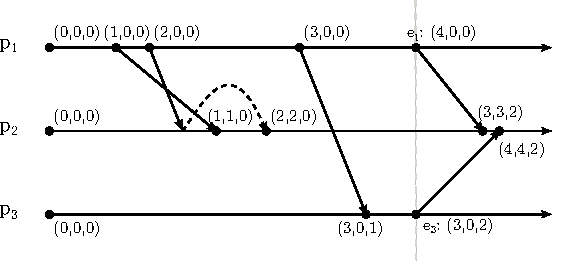
\includegraphics[width=1\textwidth]{VektorConcurr.pdf}
    \caption[Aufheben von Nachrichten]{Grafische Darstellung des Fork-Join-Event Modells bei Verwendung von Interval Tree Clocks in einem dynamischen System.}
    \label{fig:vecConcurrent}
\end{figure} 


Es kann jedoch passieren, dass durch die Vektoruhr keine Reihenfolge zwischen zwei Aktualisierungen festgestellt werden konnte, nämlich genau dann wenn $e_1 \parallel e_2$ gilt.
Diese nebenläufige Schreiboperationen, also Operationen die noch nicht abgeschlossen sind bevor Neue ausgeführt werden, stellen ein Problem für die eventual consistency dar.
Um einen Datenverlust zu vermeiden muss entschieden werden, in welcher Reihenfolge die Schreiboperationen ausgeführt werden sollen.
Die Schwierigkeit besteht jedoch darin, dass die Vektoruhr keine Aussage hierzu treffen kann.
\fig{TODO} zeigt zwei gleichzeitig aufgetretene Schreiboperationen $e_1$ und $e_3$.
Durch die Vektoruhren kann auf die Nebenläufigkeit $e_1 \parallel e_3$ getestet werden:
\begin{align*}
      C_3(e_3)[1] & \leq C_1(e_1)[1] & \wedge & & C_1(e_1)[3] & \leq C_3(e_3)[3] \\
        3         & \leq 4           & \wedge & & 0           & \leq 2
\end{align*}

Da es sich hierbei um eine wahre Aussage handelt gilt, dass $e_1$ und $e_2$ gleichzeitig aufgetreten sein müssen.
Nun muss entschieden werden wie mit so einer Situation umgegangen wird.
Da die Middelware, die in der Regel die Handhabung der Vektoruhr übernimmt, keinerlei Informationen über den Inhalt der Datenfelder oder generell über die kommunizierten Daten hat, kann sie nur den Konflikt an die Applikationsschicht melden und eine Auflösung des Konflikts anfordern.
Wie die Applikation endgültig den Konflikt löst ist stark anwendungsabhängig und unterscheidet sich von Fall zu Fall.
Eine einfache, jedoch mit Datenverlust behaftete Lösung ist es die letzte Schreiboperation zu übernehmen und die ältere zu verwerfen.

Die Amazon Datenbank unterscheidet zwischen syntaktische und schematische Konflikte.
Können die Operationen durch die Vektoruhren kausal geordnet werden, gilt der Konflikt als syntaktisch gelöst.
Ist dies nicht möglich muss er schematisch gelöst werden, also durch die Applikationsschicht.


\subsection{Aufheben alter Nachrichten}
% 1. Ereignisse müssen alle Prozesse mitgeteilt werden. Nachrichten müssen solange aufgehoben werden, bis alle die Nachricht erhalten haben. Anhand von Nachrichten der anderen Prozessen kann mit deren Vektorclock entschieden werden welche Nachrichten sie von einem selbst schon haben
% 2. Nachrichten müssen für eventual Consitiency aufgehoben werden. Daei kann es passieren, dass eine Nachricht rein kommt die bereits die alten Zustände enthält und somit die alten Nachrichten obsolete.
% 3. Matrix Clock 'fire and forget'
% http://stackoverflow.com/questions/21359184/what-do-matrix-clocks-solve-but-vector-clocks-cant
% Voraussetzung: eventual consistency
% Zeigen Ohne Matrix würde es nicht gehen
% Matrix Uhren ermöglichen GC
Anhand Vektoruhren kann entschieden werden, wann zwischengespeicherte Nachrichten gelöscht werden können.
Hierzu gibt es drei potentielle Situationen in denen, entschieden werden muss wann etwas sicher gelöscht werden kann.
Für die ersten Beiden können Vektoruhren angewendet werden und für die letzte muss eine Erweiterung von Vektoruhren heran gezogen werden.

Eine Situation in der alte Nachrichten aufgehoben werden müssen, ist gegeben wenn ein Prozess seine versandet Nachrichten aufheben muss für den Fall, dass sie neu angefordert werden.
Andere Prozesse könnten unter gewissen Umständen Nachrichten erneut anfordern, wenn diese auf die Nachricht warten.
Eine andere Möglichkeit ist es, dass eine Synchronisation der Uhren angefordert wurde und die Prozesse sich versuchen anzugleichen.
Hierzu wird jede versandte Nachricht gespeichert, inklusive der Vektoruhr zum Zeitpunkt des Versendens.
Damit der Speicherbedarf nicht ins Unendliche wächst, müssen gespeicherte Nachrichten auch wieder gelöscht werden.
Dazu muss jedoch bekannt sein, welche Nachrichten gelöscht werden können ohne einen Datenverlust zu verursachen.

Eine Möglichkeit ist es, die Vektoruhren der eingehenden Nachrichten mit den Uhren der gespeicherten Nachrichten zu vergleichen.
Erhält der Prozess eine Vektoruhr eines anderen Prozesses indem seine Vektorkomponente größer oder gleich die der gespeicherten Nachricht ist, muss der andere Prozess die alten Nachricht bekommen und verarbeitet haben.
Dies ist durch die Updatevorschriften der Vektoruhr immer gegeben.

Verschickt der Prozess $i$ zu einem gegebenen Zeitpunkt $x$ seine Nachricht und speichert diese, muss der Empfänger $j$ das Maximum zwischen seiner lokalen Uhr und der Uhr aus der Nachricht für die Komponente des Prozesses $i$ nehmen.
Nun kann der Wert in der Nachricht das Maximum sein.
In diesem Fall wird der Zeitpunkt $x$ in die lokale Uhr übernommen.
Andernfalls hat der Empfänger bereits aktuellere Nachrichten von $i$ empfangen und seine lokale Vektoruhr erhält einen Wert $>x$.

In jedem Fall wird die zu dem Senderprozess zugehörige Komponente der Vektoruhr einen größeren oder gleichen Wert haben als die gesendete Nachricht.
Schickt nun der Empfänger seinerseits eine Nachricht an den ursprünglichen Sender $i$ muss er seine lokale Vektoruhr mit anfügen.
Anhand dieser kann der Prozess $i$ bestimmen, welche Nachrichten bereits von $j$ verarbeitet wurden, nämlich alle die kleiner oder gleich der Vektoruhr von $j$ für die $i$-te Komponente sind.

Dieses Vorgehen funktioniert auch indirekt zwischen mehr als zwei Prozessen.
\fig{TODO} zeigt eine solche Situation.
Prozess $p_0$ sendet zwei Nachricht $m_1$ und $m_2$ an $p_1$.
Anschließend schickt $p_1$ eine Nachricht $m_2$ an $p_3$.
Zu diesem Zeitpunkt kennt $p_3$ den aktuellsten Stand von $p_2$ und auch $p_1$, da diese zum Zeitpunkt des Verschickens von $m_2$ von $p_2$ bekannt war.
Schickt nun $p_3$ eine Nachricht an Prozess $p_1$, kann dieser aus der Vektoruhr erschließen, dass $p_3$ die Information von Nachricht $m_1$ erhalten hat.
Sendet nun $p_2$ noch eine Nachricht an $p_1$, kann $p_1$ erkennen, dass alle im Prozess den aktuellen Zustand kennt.
Somit kann $p_1$ die gespeicherten Nachrichten $m_1$ und $m_2$ verwerfen, da das gesamte System sie bereits erhalten hat.

% TODO figure

Eine zweite Situation in der alte Nachrichten, diesmal auf der Empfängerseite, gespeichert werden, ergibt sich wenn die Auslieferung der Nachrichten kausal geordnet erfolgen soll.
Dies ist zum Beispiel der Fall bei eventual consistency, da Aktualisierungen in der selben Reihenfolge angewendet werden muss in der sie aufgetreten sind.
Sendet nun ein Prozess $p_1$ Nachrichten an einen Prozess $p_2$, können diese in beliebiger Reihenfolge bei $p_2$ ankommen, dürfen jedoch nur in der Sendereihenfolge an die Applikation übertragen werden.

Nachrichten die außerhalb der Reihenfolge angekommen sind, müssen solange gespeichert werden bis die erwartete Nachricht ankommt.
Dies kann auch Nachrichten von einem dritten Prozess betreffen, da diese kausal von den restlichen Nachrichten abhängen können.
Sobald die erwartete Nachricht eingetroffen ist, kann diese zugestellt werden und alle gespeicherten Nachrichten die nun in der Reihenfolge als nächstes kommen.

Die gespeicherten Nachrichten werden in der Regel in einer Prioritätswarteschlange (engl. \qq{priority queue}) gespeichert.
Diese ist nach den Vektoruhren der Nachrichten sortiert und ermöglicht einen effizienten Zugriff auf die gespeicherten Nachrichten.

Im Allgemeinem muss die Anwendung entscheiden, wie sie auf den Inhalt der Nachrichten reagiert.
Damit die Anwendung richtig entscheiden kann, müssen alle Nachrichten zugestellt werden.
Ist dies nicht gegeben, ist nicht garantiert, dass die Anwendung in jeden Fall korrekt funktioniert.
Es gibt jedoch Anwendungsfälle, wie zum Beispiel verteilte Datenbanken, bei denen nur die letzte Aktualisierung von Relevanz ist.
In diesem Fall können alle gespeicherten Nachrichten verworfen werden, wenn eine aktuellere Nachricht empfangen wurde.
Dies stellt eine mögliche Optimierung dar, da nicht alle Nachrichten sondern nur eine, die Aktuellste, der Anwendung gemeldet werden muss.

\fig{TODO} zeigt eine Situation in der die zu erst verschickte Nachricht $m_1$ von $p_1$ von den beiden Nachrichten $m_2$ und $m_3$ überholt wurde und somit als letztes bei $p_2$ angekommen ist.
Eine Möglichkeit ist es nun, dass $p_2$ die Nachrichten $m_2$ und $m_3$ bis zum Empfangen von $m_1$ aufhebt und die Nachrichten in der korrekten Reihenfolge der Anwendung zustellt.
Alternativ könnte $p_2$ aber auch beim Empfangen von $m_2$ und $m_3$ diese direkt Zustellen und $m_1$ verwerfen, da bereits aktuellere Nachrichten empfangen wurden und der Inhalt von $m_1$ bereits bekannt oder obsolete ist.

% TODO figure

Der letzte Anwendungsfall ist Garbage Collection innerhalb des verteilten Systems.
Angenommen ein Prozess möchte eine Nachricht verschicken und deren Information sofort wieder verwerfen.
Natürlich darf die Information nur gelöscht werden, wenn alle Prozesse diese erhalten haben.
Dabei soll es keine Rolle spielen ob die Information direkt an alle Prozesse oder auch über Umwege indirekt verteilt wird.
Hierzu müsste der Prozess die Vektoruhren der anderen Prozesse kennen.
Dies verhält sich ähnlich zu dem ersten beschriebenen Anwendungsfall.

Ein Lösung für dieses Problem stellen Matrixuhren dar.
Vektoruhren können als Wissenstand interpretiert werden.
$VC_a(x)[i]$ beschreibt was der Prozess $a$ über den Prozess $i$ weiß, zu dem Zeitpunkt als $e$ eingetreten ist.
Es liegt nahe dieses Wissen über andere Prozesse leicht erweitert werden kann, indem eine höher dimensionale Struktur verwendet wird.
So kann der Vektor zu einer Matrix erweitert werden und als Liste von Vektoren betrachtet werden.
Durch $MC_a(x)[i,j]$ kann der Prozess $a$ erfahren, was der Prozess $i$ über Prozess $j$ weiß, zum Zeitpunkt $e$.
Diese Erweiterung wird nach ihrer Struktur als Matrixuhr bezeichnet.
Gilt nun zum Beispiel für alle $i$ das $MC_j(e)[i, j] > k$, kann nun der Prozess $j$ erschließen, dass jedem Prozess bekannt ist, dass sein aktueller Zustand größer $k$ ist.
Die Updateregeln von Matrixuhren verhalten sich ähnlich zu denen von Vektoruhren \cite{garg2005concurrent}.

In unserem oben gegebenen Szenario können nun Matrixuhren sinnvoll eingesetzt werden.
Angenommen die Nachricht wurde zu dem Zeitpunkt $MC[i][i]=k$ von Prozess $i$ verschickt, dann muss
\begin{equation*}
\forall j \colon MC[j][i] \geq k
\end{equation*}
erfüllt sein, damit $i$ die Nachricht löschen kann.
Die obige Bedingung impliziert, dass die $i$-te Komponente der Vektoruhren aller Prozesse $j$ größer oder gleich $k$ sind.
Somit hat sich die Information von Prozess $i$ durch das komplette System verteilt und kann somit gelöscht werden \cite{garg2005concurrent}.


